% --- Program Section ---

\newprogram{Program 6}{Construct a Graph class with kruskal-mst() -> List[Edge] and prim-mst() -> List[Edge]
methods that process edge-weighted graph structures and return the MST edge set.}

\subsection*{Code}
\begin{lstlisting}[language=Python]
from dataclasses import dataclass
from typing import List
import heapq


@dataclass
class Edge:
    u: int
    v: int
    weight: int


class Graph:
    def __init__(self, vertices: int):
        self.vertices = vertices
        self.edges = []

    def add_edge(self, u: int, v: int, weight: int):
        self.edges.append(Edge(u, v, weight))

    # -------------------------
    # Kruskal's Algorithm
    # -------------------------
    def kruskal_mst(self) -> List[Edge]:
        parent = list(range(self.vertices))

        def find(x):
            if parent[x] != x:
                parent[x] = find(parent[x])
            return parent[x]

        def union(a, b):
            root_a = find(a)
            root_b = find(b)

            if root_a != root_b:
                parent[root_b] = root_a
                return True

            return False

        # Sort edges by weight
        edges = sorted(self.edges, key=lambda e: e.weight)

        mst = []

        for edge in edges:
            if union(edge.u, edge.v):
                mst.append(edge)

                if len(mst) == self.vertices - 1:
                    break

        return mst

    # -------------------------
    # Prim's Algorithm
    # -------------------------
    def prim_mst(self) -> List[Edge]:
        if self.vertices == 0:
            return []

        # Adjacency list
        graph = [[] for _ in range(self.vertices)]

        for edge in self.edges:
            graph[edge.u].append((edge.weight, edge.u, edge.v))
            graph[edge.v].append((edge.weight, edge.v, edge.u))

        visited = [False] * self.vertices
        heap = [(0, -1, 0)]

        mst = []

        while heap and len(mst) < self.vertices - 1:
            weight, parent, vertex = heapq.heappop(heap)

            if visited[vertex]:
                continue

            visited[vertex] = True

            if parent != -1:
                mst.append(Edge(parent, vertex, weight))

            for next_weight, u, v in graph[vertex]:
                if not visited[v]:
                    heapq.heappush(heap, (next_weight, vertex, v))

        return mst


# -------------------------
# Example
# -------------------------

g = Graph(4)

g.add_edge(0, 1, 10)
g.add_edge(0, 2, 6)
g.add_edge(0, 3, 5)
g.add_edge(1, 3, 15)
g.add_edge(2, 3, 4)

kruskal = g.kruskal_mst()
prim = g.prim_mst()

print("Kruskal MST:")
for edge in kruskal:
    print(edge.u, "-", edge.v, ":", edge.weight)

print("\nPrim MST:")
for edge in prim:
    print(edge.u, "-", edge.v, ":", edge.weight)
\end{lstlisting}

\subsection*{Output}
\begin{center}
    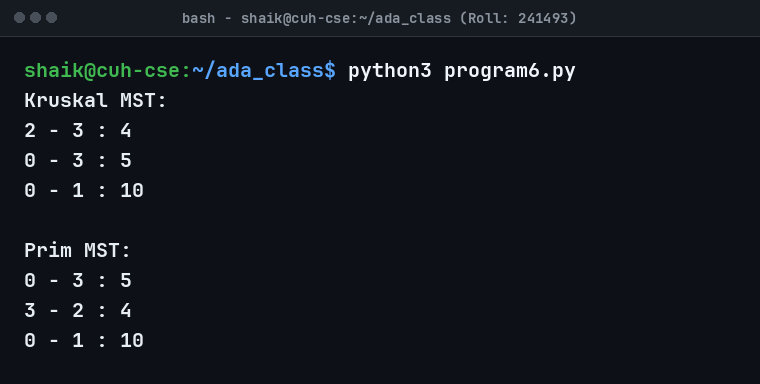
\includegraphics[width=0.88\textwidth]{Images/output_screenshot6.png}
\end{center}

\subsection*{GitHub Scan Code}
\begin{center}
    \begin{minipage}{0.3\textwidth}
        \centering
        % Generates a 2.5cm high QR code directly linking to the code file
        \qrcode[height=3.5cm]{https://github.com/gytdrop/ada_class/blob/main/program6.py} \\[0.2cm]
        \scriptsize\ttfamily Scan to view source code 
    \end{minipage}
\end{center}


% Add a horizontal line that indicates the END of the program.
\vspace{1cm}
\begin{center}
    \rule{1\textwidth}{1pt} % Clean, centered 1pt thick horizontal line
\end{center}